\section{Příklad 4}
% Jako parametr zadejte skupinu (A-H)
\ctvrtyZadani{B}

\large{\textbf{Řešení:}}

%%% Krok 1 - Vypočítanie uhlovej rýchlosti a impedancií
\begin{center}
    Nejprve zapíšeme tři důležité rovnice.
    \begin{gather*}
    \omega = 2 \pi f\\\\
    Z_L = j \omega L \\\\
    Z_C = \frac{1}{j \omega C} \\
    \end{gather*}
    
    Vypočítáme úhlovou rychlost $\omega$ a impedance jednotlivých cívek a kondenzátorů.
    
    \begin{gather*}
        \omega = 2 \pi 80 = 160 \pi \\\\
        Z_{L_1} = j \times 160 \pi  \times 100 = j50.26548246 \Omega \\
        Z_{L_2} = j \times 160 \pi \times 85 = j42.72566009 \Omega \\\\
        Z_{C_1} = \frac{1}{j \times 160 \pi \times 220} = -j9.04289449 \Omega \\
        Z_{C_2} = \frac{1}{j \times 160 \pi \times 95} = -j20.94143988 \Omega
    \end{gather*}
    
\end{center}

\newpage

%%% Krok 2 - Zostavenie rovnice pre slučkové prúdy
\begin{center}
    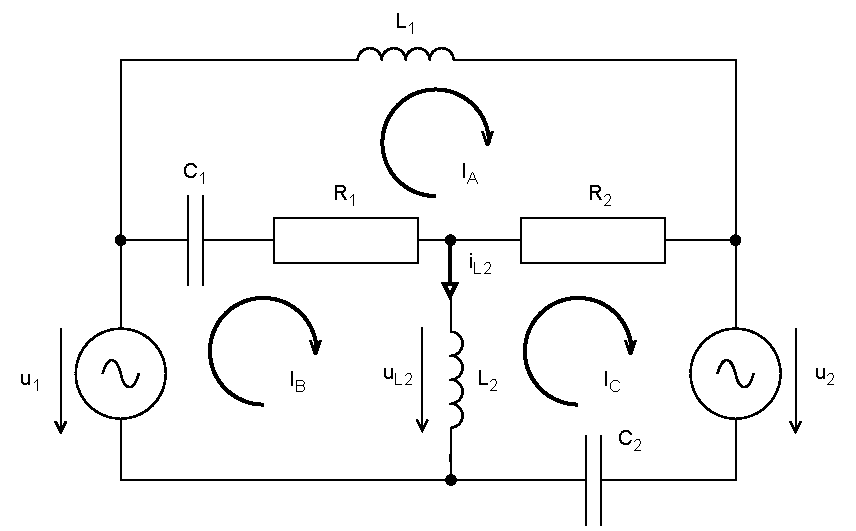
\includegraphics[scale=0.8,keepaspectratio]{fig/solutions/04-sol/04-step1.pdf} \\
    Obr.4.1 - Sestavíme rovnice pro smyčkové proudy
\end{center}

\begin{gather*}
    I_A: I_A(Z_{L_1} + Z_{C_1} + R_1 + R_2) + I_B(-Z_{C_1} - R_1) + I_C(-R_2) = 0 \\\\
    I_B: I_A(-Z_{C_1} - R_1) + I_B(Z_{C_1} + R_1 + Z_{L_2}) + I_C(-Z_{L_2}) = u_1 \\\\
    I_C: I_A(-R_2) + I_B(-Z_{L_2}) + I_C(Z_{C_2} + Z_{L_2} + R_2) = -u_2 \\
\end{gather*}

\noindent Vytvoříme matici rovnic:
\begin{gather*}
    \begin{pmatrix}
    Z_{L_1} + Z_{C_1} + R_1 + R_2 & -Z_{C_1} - R_1 & -R_2 \\
    -Z_{C_1} - R_1 & Z_{C_1} + R_1 + Z_{L_2} & -Z_{L_2} \\
    -R_2 & -Z_{L_2} & Z_{C_2} + Z_{L_2} + R_2
    \end{pmatrix}
    \times
    \begin{pmatrix}
    I_A \\
    I_B \\
    I_C \\
    \end{pmatrix}
    =
    \begin{pmatrix}
    0 \\
    u_1 \\
    -u_2
    \end{pmatrix}
\end{gather*}
\\

Pomocí Cramerova a Sarussova pravidla najdeme hodnoty $I_A$ a $I_C$:
\begin{gather*}
    M = 
    \begin{vmatrix}
    Z_{L_1} + Z_{C_1} + R_1 + R_2 & -Z_{C_1} - R_1 & -R_2 \\
    -Z_{C_1} - R_1 & Z_{C_1} + R_1 + Z_{L_2} & -Z_{L_2} \\
    -R_2 & -Z_{L_2} & Z_{C_2} + Z_{L_2} + R_2
    \end{vmatrix}
    =
    -17018.55524910 + j51623.75347964
\end{gather*}

\begin{gather*}
    M_{I_B} = 
    \begin{vmatrix}
    Z_{L_1} + Z_{C_1} + R_1 + R_2 & 0 & -R_2 \\
    -Z_{C_1} - R_1 & u1 & -Z_{L_2} \\
    -R_2 & -u2 & Z_{C_2} + Z_{L_2} + R_2
    \end{vmatrix}
    =
    4919.04525774 - j1531.43788987
\end{gather*}

\begin{gather*}
    M_{I_C} = 
    \begin{vmatrix}
    Z_{L_1} + Z_{C_1} + R_1 + R_2 & -Z_{C_1} - R_1 & 0 \\
    -Z_{C_1} - R_1 & Z_{C_1} + R_1 + Z_{L_2} & u1 \\
    -R_2 & -Z_{L_2} & -u2
    \end{vmatrix}
    =
    1374.34274444 - j4162.12871793
\end{gather*}

\begin{gather*}
    I_B = \frac{M_{I_B}}{M} = -0.05509079 - j0.07712495 A \\
    I_C = \frac{M_{I_C}}{M} = -0.08063716 - j0.00003903 A
\end{gather*}
\\
Proud, který prochází kondenzátorem $L_2$, lze zjistit pomocí rovnice:
\begin{gather*}
    I_{L_2} = I_B - I_C = 0.02554637 - j0.07708593 A
\end{gather*}
\\
Napětí $|U_{L 2}|$ vypočítáme pomocí Ohmova zákona a vypočítáme $\boldsymbol{|U_{L_2}|}$ a $\boldsymbol{\varphi_{L_2}}$:
\begin{gather*}
    u_{L_2} = Z_{L_2} \times I_{L_2} = 3.29354712 + j1.09148570 V \\
    \boldsymbol{|U_{L_2}|} = \sqrt{Re(u_{L_2})^2 + Im(u_{L_2})^2} = \textbf{3.46969647V} \\
    \boldsymbol{\varphi_{L_2}} =
    \arctan \frac{Im(u_{L_2})}{Re(u_{L_2})} =
    \arctan \frac{1.09148570}{3.29354712} =
    \textbf{0.32001069 rad} = \textbf{18.33526199$^{\circ}$}
\end{gather*}